%--------------------------------------------------------------------------------
% CONFIGURATION DU DOCUMENT
%--------------------------------------------------------------------------------

\documentclass[a4paper,12pt]{report}

\usepackage[french]{babel}
\usepackage[utf8]{inputenc}
\usepackage[T1]{fontenc}
\usepackage{mathptmx}
\usepackage[most]{tcolorbox}
\usepackage[a4paper, left=2.5cm, right=2.5cm, top=2.5cm, bottom=2.5cm]{geometry}
\usepackage{graphicx}
\usepackage{lipsum}
\usepackage{hyperref}

% Pour les arbres
\usepackage{tikz} 
\usetikzlibrary{shapes.geometric, trees}

\setlength{\textfloatsep}{10pt}

\begin{document}





%--------------------------------------------------------------------------------
% PAGE DE GARDE
%--------------------------------------------------------------------------------

\begin{titlepage}
    \centering

    %----------------------------------
    % Informations sur l'université
    %----------------------------------

    {\large Faculté des Sciences et Ingénierie - Sorbonne Université}\\[0.3cm]
    {\large Master Informatique parcours ANDROIDE}\\[1cm]
    
\includegraphics[width=0.3\textwidth]{../images/logo_SU.png}\\[1.5cm]


    %----------------------------------
    % Informations sur le projet
    %----------------------------------

    \vspace{1.5cm}

    {\LARGE COMPLEX - Complexité, algorithmes randomisés et approchés}\\[1cm]
    {\Large Rapport de projet}\\[2cm]
    \rule{\linewidth}{0.5mm} \\[1cm]
    {\Huge \textbf{Arbres Cartésien et Algorithmes associés}} \\[0.4cm]
    \rule{\linewidth}{0.5mm} \\[2cm]
    

    %----------------------------------
    % Informations sur nous
    %----------------------------------

    \begin{flushleft}
        \textbf{Réalisé par :} \\[0.3cm]
        PINHO FERNANDES Enzo \\[0.2cm]
        BEN SALAH Adel \\[2cm]
    \end{flushleft}
    

    %----------------------------------
    % Date
    %----------------------------------

    \vfill
    {\large Novembre 2024}\\
    
\end{titlepage}





%--------------------------------------------------------------------------------
% Table des matières
%--------------------------------------------------------------------------------

\tableofcontents





%--------------------------------------------------------------------------------
% Page d'introduction
%--------------------------------------------------------------------------------

\newpage

\chapter*{Introduction du projet}
\addcontentsline{toc}{chapter}{Introduction du projet}

Les arbres cartésiens sont une structure de données qui combine les propriétés des arbres binaires de recherche et des tas. Ils ont été proposés par Jean Vuillemin en 1980. Voici un aperçu de leur structure et de leur fonctionnement :\\[-0.4cm]

\textbf{Structure}
\begin{itemize}
    \item \textbf{Noeuds :} chaque noeud d'un arbre cartésien contient une clé (qui respecte l'ordre d'un arbre binaire de recherche) et une priorité (qui respecte l'ordre d'un tas).
    \item \textbf{Arbre binaire de recherche :} les noeuds sont organisés de manière à ce que, pour tout noeud, les clés de son sous-arbre gauche soient inférieures à sa clé, et celles de son sous-arbre droit soient supérieures.
    \item \textbf{Tas :} les noeuds sont également organisés selon la priorité, de sorte qu'un parent ait toujours une priorité inférieure à celle de ses enfants.
\end{itemize}

\begin{figure}[!h]
    \centering
    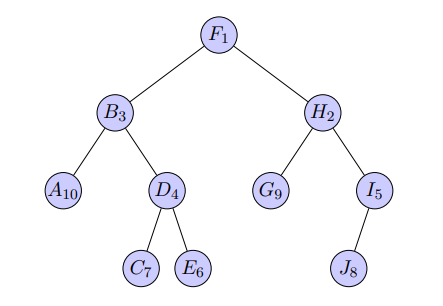
\includegraphics[width=0.5\textwidth]{../images/figure1.png}
    \caption{Exemple d'arbre cartésien contenant les clés de \{A,B,\dots,J\} avec les valeurs de priorités dans \{1,\dots,10\} données en indice.}
\end{figure}

\textbf{Propriétés}
\begin{itemize}
    \item \textbf{Équilibre probabiliste :} Les arbres cartésiens maintiennent une structure équilibrée de manière \textbf{probabiliste}. Cela signifie que les opérations d'insertion, de suppression et de recherche ont une complexité en temps moyenne de \( O(\log n) \) même si dans le pire des cas, cela peut atteindre \( O(n) \) (où \( n \) désigne le nombre de noeuds de l'arbre cartésien).
    \item \textbf{Insertion et suppression :} Lors de l'insertion, un nouveau noeud est placé comme un noeud feuille dans l'arbre binaire de recherche. Puis, si sa priorité est inférieure à celle de son parent, il est "élevé" à travers des rotations jusqu'à ce que l'ordre du tas soit respecté (\textit{cf.} Exercice 3).
    \item \textbf{Recherche :} La recherche d'une clé suit les règles d'un arbre binaire de recherche, ce qui la rend efficace.
\end{itemize}

\newpage

Les arbres cartésiens sont utilisés dans diverses applications où une structure de données dynamique et équilibrée est nécessaire, comme la gestion de fichiers, les bases de données et les algorithmes de traitement d'événements. Le but de ce projet est d'implanter et d'analyser cette structure de données et d'effectuer des tests d'efficacités.





%--------------------------------------------------------------------------------
% Exercice 1 : Arbres cartésiens - Premières propriétés
%--------------------------------------------------------------------------------

\newpage

\renewcommand{\chaptername}{Exercice}
\chapter{Arbres cartésiens - Premières propriétés}



%--------------------------------------------------------------------------------
% Question 1.a
%--------------------------------------------------------------------------------

\addcontentsline{toc}{section}{a. Construction de l'arbre cartésien}

\textbf{1.a]} Construire un arbre cartésien dont les noeuds sont donnés par la liste suivante (la lettre représentant la clé du noeud et l'entier sa priorité) :
\[
(A:5), (B:3), (C:8), (D:2), (E:6), (F:7), (G:9), (H:1), (I:10), (J:12)
\]
Existe-t-il plusieurs solutions ? Qu'en est-il pour un arbre cartésien dont toutes les priorités sont différentes (ce que nous ferons dans toute la suite du projet). Justifier votre réponse.\\



\begin{tcolorbox}[colback=gray!10, colframe=blue!30, coltitle=black, title=Réponse à la 1.a - 1/2]
    Arbre cartésien de la liste précédente :\\

    \begin{center}
        \begin{tikzpicture}[every node/.style = {minimum width = 2em, draw, circle}, level/.style = {sibling distance = 50mm/#1}]
            \node {\(H_1\)}
            child {   
                node {\(D_2\)} 
                child {   
                    node {\(B_3\)}
                    child {
                        node {\(A_5\)}
                    }
                    child {
                        node {\(C_8\)}
                    }
                }
                child {
                    node {\(E_6\)}
                    child {edge from parent[draw = none]}
                    child {
                        node {\(F_7\)}
                        child {edge from parent[draw = none]}
                        child {
                            node {\(G _9\)}
                        }
                    }
                }
            }
            child {
                node {\(I_{10}\)}
                child {edge from parent[draw = none]}
                child {
                    node {\(J_{12}\)}
                }
            };
        \end{tikzpicture}
    \end{center}

    Il n'existe pas plusieurs solutions, et cela est vrai également pour tout arbre cartésien dont toutes les priorités sont différentes, grâce aux propriétés d'un arbre de recherche binaire et d'un tas.

    \vspace{0.5cm}
    \hrule
    \vspace{0.5cm}

    En effet, dans un arbre cartésien, la \textbf{racine} doit être le noeud avec \textbf{la priorité la plus faible} parmi tous les noeuds par la propriété du tas. Par conséquent, il n'y a qu'une possibilité, le choix de la racine est unique.

\end{tcolorbox}
\begin{tcolorbox}[colback=gray!10, colframe=blue!30, coltitle=black, title=Réponse à la 1.a - 2/2]

    Une fois cela fait, l'ensemble des autres noeuds de priorité inférieure seront divisés en deux sous-ensembles selon leur clé, d'après la propriété d'un arbre de recherche binaire :\\[-0.4cm]
    \begin{itemize}
        \item Le sous-arbre gauche contiendra tous les noeuds ayant des clés inférieures à celle de la racine.
        \item Le sous-arbre droit contiendra tous les noeuds ayant des clés supérieures à celle de la racine.
    \end{itemize}

    \vspace{0.5cm}

    Ces deux sous-ensembles sont indépendants l'un de l'autre, et surtout uniques. Chacun de ces sous-ensembles doivent représenter eux-même un arbre cartésien.\\

    On suivra le même raisonnement récursivement sur les sous-ensembles gauche et droit :\\[-0.4cm]
    \begin{itemize}
        \item On choisit le noeud du premier sous-ensemble avec la priorité la plus faible comme racine.
        \item On choisit le noeud du second sous-ensemble avec la priorité la plus faible comme racine.
    \end{itemize}

    \vspace{0.5cm}

    Et on recommence jusqu'à que tous les noeuds soient placés dans l'arbre cartésien.

    \vspace{0.5cm}
    \hrule
    \vspace{0.5cm}

    En conclusion, \textbf{tout arbre cartésien est unique} (si toutes les priorités sont différentes) puisque chaque décision de construction est unique, alias :\\[-0.4cm]
    \begin{itemize}
        \item Le choix de la racine, de par sa priorité la plus faible de son sous-ensemble, grâce à la propriété du tas.
        \item Le choix des deux sous-ensembles, de par les clés des noeuds, grâce à la propriété des arbres de recherche binaire. 
    \end{itemize}

\end{tcolorbox}



%--------------------------------------------------------------------------------
% Question 1.b
%--------------------------------------------------------------------------------

\newpage
\addcontentsline{toc}{section}{b. Insertion de noeuds dans un ordre prédéfini}

\textbf{1.b]} Considérer l'arbre binaire de recherche construit en insérant dans l'ordre les noeuds dont les clés sont les suivantes : \( H, D, B, A, E, F, C, G, I \) et \( J \) et comparer à l'arbre cartésien de la question précédente. Généraliser et démontrer ce résultat pour un arbre cartésien général (dont les priorités sont différentes).\\



\begin{tcolorbox}[colback=gray!10, colframe=blue!30, coltitle=black, title=Réponse à la 1.b - 1/1]

    L'arbre issu de l'insertion de ces noeuds, dans cet ordre, donne exactement le même arbre cartésien de la question précédente.\\

    \begin{center}
        \begin{tikzpicture}[every node/.style = {minimum width = 2em, draw, circle}, level/.style = {sibling distance = 50mm/#1}]
            \node {\(H\)}
            child {   
                node {\(D\)} 
                child {   
                    node {\(B\)}
                    child {
                        node {\(A\)}
                    }
                    child {
                        node {\(C\)}
                    }
                }
                child {
                    node {\(E\)}
                    child {edge from parent[draw = none]}
                    child {
                        node {\(F\)}
                        child {edge from parent[draw = none]}
                        child {
                            node {\(G \)}
                        }
                    }
                }
            }
            child {
                node {\(I\)}
                child {edge from parent[draw = none]}
                child {
                    node {\(J\)}
                }
            };
        \end{tikzpicture}
    \end{center}

    Nous avons cette corrélation entre les deux arbres parce que nous avons inséré les noeuds selon leur priorité (en ordre croissant) dans l'arbre cartésien.

    \vspace{0.5cm}
    \hrule
    \vspace{0.5cm}

    On peut généraliser ce résultat en : un arbre cartésien est un ABR où nous avons inséré les noeuds dans l'ordre croissant de leur priorité (si elles sont toutes différentes).\\

    En effet, trois propriétés sont visibles dans ce cas précis :\\[-0.4cm]
    \begin{itemize}
        \item La racine des deux arbres sont les mêmes, alias le noeud dont la priorité est la plus faible.
        \item La propriété de l'ABR est respecté dans les deux cas, étant donné la nature des arbres.
        \item La propriété du tas est respecté pour l'arbre cartésien bien évidemment, mais également pour cet ABR. En effet, pour ce dernier, on insère les noeuds dans l'ordre croissant de leur priorité. D'après l'algorithme d'insertion de ce dernier, il deviendra forcément une des feuilles de l'arbre à la fin de l'insertion, et il n'y a pas de rotation. Par conséquent, tout parent de cet arbre aura une priorité plus faible que leurs enfants.
    \end{itemize}

    \vspace{0.5cm}

    Étant donné que tout arbre respectant les propriétés d'un ABR et d'un tas est unique, et que dans ce cas précis, nos deux arbres respectent ces propriétés et possèdent la même racine, alors... Ils sont égaux, dû à leur unicité.

\end{tcolorbox}



%--------------------------------------------------------------------------------
% Question 1.c
%--------------------------------------------------------------------------------

\newpage
\addcontentsline{toc}{section}{c. Implémentation de la structure de données d'un noeud}

\textbf{1.c]} Programmer la structure de données d'un noeud (contenant la clé et la priorité, le pointeur vers le fils gauche, le pointeur vers le fils droit) avec les constructeurs et les fonctions associés.



\begin{tcolorbox}[colback=gray!10, colframe=blue!30, coltitle=black, title=Réponse à la 1.c - 1/1]

    Nous avons décidé d'implémenter nos différentes structures de données en JAVA, pour sa simplicité quant à l'utilisateur des pointeurs ainsi que de la mémoire.\\

    En effet, le garbage collector s'occupe de libérer la mémoire dès qu'un objet n'est plus référencé, ce qui nous sera très pratique au moment de la suppression des noeuds.\\

    L'implémentation se trouve dans le fichier : \href{./src/Node.java}{./src/Node.java}

\end{tcolorbox}



%--------------------------------------------------------------------------------
% Question 1.d
%--------------------------------------------------------------------------------

\vspace{1.5cm}
\addcontentsline{toc}{section}{d. Implémentation de la structure de données d'un arbre cartésien}

\textbf{1.d]} Programmer la structure de données d'un arbre cartésien (avec au minimum un constructeur pour l'arbre cartésien vide, une fonction pour tester si un arbre cartésien est vide, pour accéder au fils droit/gauche d'un noeud donné).

\begin{tcolorbox}[colback=gray!10, colframe=blue!30, coltitle=black, title=Réponse à la 1.d - 1/1]

    L'implémentation se trouve dans le fichier : \href{./src/CartesianTree.java}{./src/CartesianTree.java}

\end{tcolorbox}



%--------------------------------------------------------------------------------
% Question 1.e
%--------------------------------------------------------------------------------

\vspace{1.5cm}
\addcontentsline{toc}{section}{e. Construction manuelle de l'arbre cartésien de la question 1.a}

\textbf{1.e]} Avec votre implantation, construire "manuellement" l'arbre cartésien de la question 1.a.

\begin{tcolorbox}[colback=gray!10, colframe=blue!30, coltitle=black, title=Réponse à la 1.e - 1/1]

    La construction de l'arbre se trouve dans le fichier test : \href{./test/Exo\_1\_e.java}{./test/Exo\_1\_e.java}\\

    Le test "testTreeStructure" affiche l'arbre obtenu dans la console de débogage.
\end{tcolorbox}





%--------------------------------------------------------------------------------
% Exercice 2 : Recherche dans un arbre cartésien
%--------------------------------------------------------------------------------

\newpage

\renewcommand{\chaptername}{Exercice}
\chapter{Recherche dans un arbre cartésien}



%--------------------------------------------------------------------------------
% Question 2.a
%--------------------------------------------------------------------------------

\addcontentsline{toc}{section}{a. Implémentation de l'algorithme de recherche d'un noeud}

\textbf{2.a]} Implanter l'algorithme de recherche d'un noeud contenant une clé donnée dans un arbre cartésien. L'algorithme est identique à celui de recherche dans un arbre binaire de recherche.



\begin{tcolorbox}[colback=gray!10, colframe=blue!30, coltitle=black, title=Réponse à la 2.a - 1/1]

    Les méthodes \texttt{searchKey} et \texttt{searchKeyRec} dans le fichier \href{./src/CartesianTree.java}{./src/CartesianTree.java} correspondent à l'implantation de l'algorithme de recherche de noeud. (l.60-85)

\end{tcolorbox}



%--------------------------------------------------------------------------------
% Question 2.b
%--------------------------------------------------------------------------------

\vspace{1.5cm}
\addcontentsline{toc}{section}{b. Complexité de l'algorithme de recherche de noeud}

\textbf{2.b]} Donner la complexité de cet algorithme en fonction de la profondeur du noeud recherché (en cas de recherche fructueuse) ou de la profondeur de son successeur ou prédécesseur du noeud recherché (en cas de recherche infructueuse).



\begin{tcolorbox}[colback=gray!10, colframe=blue!30, coltitle=black, title=Réponse à la 2.b - 1/2]

    L'algorithme de recherche d'un noeud dans un arbre cartésien est le même que celui dans un ABR.\\\\[-0.4cm]

    Lors de la recherche, à chaque itération, on identifie trois cas :
    \begin{itemize}
        \item Si la clé recherchée est la clé du noeud courant, on a trouvé le noeud.
        \item Si la clé recherchée est inférieure à celle du noeud courant, on continue la recherche chez le fils gauche.
        \item Si la clé recherché est supérieure à celle du noeud courant, on continue la recherche chez le fils droit.
    \end{itemize}

    \vspace{0.5cm}

    En toute logique, la complexité de la recherche dépendra donc du nombre de noeuds parcourus depuis la racine, jusqu'au noeud recherché si la recherche est fructueuse, sinon, jusqu'à une feuille en cas de recherche infructueuse.\\

    Posons \( d(x) \) la profondeur du noeud \( x \) étant soit le noeud recherché en cas de recherche fructueuse, sinon la feuille atteinte. Alors la complexité de la recherche est en \( O(d(x)) \).\\
\end{tcolorbox}
\begin{tcolorbox}[colback=gray!10, colframe=blue!30, coltitle=black, title=Réponse à la 2.b - 2/2]

    Mais ce n'est pas tout, on peut distinguer deux cas :
    \begin{itemize}
        \item \textbf{Le cas moyen :} Quand l'arbre cartésien est "relativement équilibré", alors la profondeur moyenne d'un noeud est environ à \( O(\log n) \), \( n \) étant le nombre de noeuds de l'arbre. Ce sera donc la complexité de la recherche dans le cas d'un arbre cartésien dont les ensembles de clés et de priorités sont bien répartis.
        \item \textbf{Le cas critique :} Quand l'arbre est déséquilibré, par exemple un arbre qui représente une liste, alors la profondeur serait en \( O(n) \). Ce sera donc la complexité dans le pire cas, où l'ensembles de clés et de priorités sont mal répartis.
    \end{itemize}

    \vspace{0.5cm}
    \hrule
    \vspace{0.5cm}

    En conclusion, on aura comme complexité pour un arbre cartésien à \( n \) noeuds :
    \begin{itemize}
        \item \textbf{S'il est équilibré :} \( O(\log n) \)
        \item \textbf{S'il est déséquilibré :} \( O(n) \)
    \end{itemize}

\end{tcolorbox}





%--------------------------------------------------------------------------------
% Exercice 3 : Insertion dans un arbre cartésien
%--------------------------------------------------------------------------------

\newpage

\renewcommand{\chaptername}{Exercice}
\chapter{Insertion dans un arbre cartésien}



%--------------------------------------------------------------------------------
% Question 3.a
%--------------------------------------------------------------------------------

\addcontentsline{toc}{section}{a. Violation de la propriété du tas lors de l'insertion (ABR)}

\textbf{3.a]} Montrer, sur l'exemple de la question 1.a. que l'insertion d'un noeud dans un arbre cartésien en suivant la méthode d'insertion dans un arbre binaire de recherche, peut résulter en un arbre qui ne vérifie plus la propriété de tas.



\begin{tcolorbox}[colback=gray!10, colframe=blue!30, coltitle=black, title=Réponse à la 3.a - 1/2]

    Prenons l'exemple de la question 1.a. Pour rappel, l'arbre cartésien est ce dernier :\\

    \begin{center}
        \begin{tikzpicture}[every node/.style = {minimum width = 2em, draw, circle}, level/.style = {sibling distance = 50mm/#1}]
            \node {\(H_1\)}
            child {   
                node {\(D_2\)} 
                child {   
                    node {\(B_3\)}
                    child {
                        node {\(A_5\)}
                    }
                    child {
                        node {\(C_8\)}
                    }
                }
                child {
                    node {\(E_6\)}
                    child {edge from parent[draw = none]}
                    child {
                        node {\(F_7\)}
                        child {edge from parent[draw = none]}
                        child {
                            node {\(G _9\)}
                        }
                    }
                }
            }
            child {
                node {\(I_{10}\)}
                child {edge from parent[draw = none]}
                child {
                    node {\(J_{12}\)}
                }
            };
        \end{tikzpicture}
    \end{center}

\end{tcolorbox}
\begin{tcolorbox}[colback=gray!10, colframe=blue!30, coltitle=black, title=Réponse à la 3.a - 2/2]

    Essayons d'insérer le noeud (Z : 11) suivant l'algorithme d'insertion d'un ABR. Le résultat sera :\\

    \begin{center}
        \begin{tikzpicture}[every node/.style = {minimum width = 2em, draw, circle}, level/.style = {sibling distance = 50mm/#1}]
            \node {\(H_1\)}
            child {   
                node {\(D_2\)} 
                child {   
                    node {\(B_3\)}
                    child {
                        node {\(A_5\)}
                    }
                    child {
                        node {\(C_8\)}
                    }
                }
                child {
                    node {\(E_6\)}
                    child {edge from parent[draw = none]}
                    child {
                        node {\(F_7\)}
                        child {edge from parent[draw = none]}
                        child {
                            node {\(G _9\)}
                        }
                    }
                }
            }
            child {
                node {\(I_{10}\)}
                child {edge from parent[draw = none]}
                child {
                    node {\(J_{12}\)}
                    child {edge from parent[draw = none]}
                    child {
                        node {\(Z_{11}\)}
                    }
                }
            };
        \end{tikzpicture}
    \end{center}

    \vspace{0.5cm}

    Nous voyons bien que cet arbre ne respecte pas les propriétés d'un arbre cartésien, étant donné qu'un parent a une priorité plus grande qu'un de ses fils, ici (J : 12) alias le parent de (Z : 11).

    \vspace{0.5cm}
    \hrule
    \vspace{0.5cm}

    Par conséquent, l'insertion d'un noeud dans un arbre cartésien en suivant la méthode d'insertion dans un arbre binaire de recherche peut résultat en un arbre qui ne vérifie plus la propriété du tas.

\end{tcolorbox}



%--------------------------------------------------------------------------------
% Question 3.b
%--------------------------------------------------------------------------------

\newpage

Pour réparer cela, l'insertion dans un arbre cartésien va se faire arbre cartésien va se faire initialement comme dans un arbre binaire de recherche mais devra effectuer des \textit{rotations} d'arbre (voir le diagrame suivant pour une rotation au noeud \( x \)) pour rétablir la propriété du tas.\\
\begin{center}
    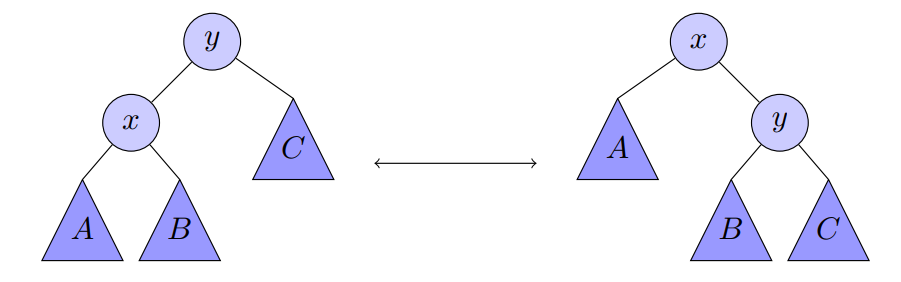
\includegraphics[width=0.7\textwidth]{../images/rotationExplication.png}\\[-0.5cm]
\end{center}

Une telle rotation préserve la propriété d'arbre binaire mais permet de rétablir la propriété de tas. Désormais pour insérer un noeud \( z \) dans un arbre cartésien, il sera inséré comme dans un arbre binaire de recherche mais une fois cela effectué, tant que sa priorité est inférieure à celle de son noeud parent, effectuer une rotation au noeud \( z \). Chaque rotation diminue la profondeur du noeud \( z \) de 1 et augmente celle de son parent de 1. Les rotations peuvent être effectuées en temps constant puisqu'il s'agit simplement de manipulation de pointeurs.

\vspace{2cm}

\addcontentsline{toc}{section}{b. Complexité de l'algorithme d'insertion d'un arbre cartésien}

\textbf{3.b]} Donnez la complexité de cet algorithme en fonction de la profondeur de son prédécesseur.



\begin{tcolorbox}[colback=gray!10, colframe=blue!30, coltitle=black, title=Réponse à la 3.b - 1/2]

    L'insertion dans un arbre cartésien suit deux étapes :\\[-0.4cm]
    \begin{itemize}
        \item L'insertion classique dans un arbre binaire de recherche.
        \item La succession de rotations jusqu'à que la propriété du tas soit respectée.
    \end{itemize}

    \vspace{0.5cm}
    \hrule
    \vspace{0.5cm}

    Posons \( x \) le noeud à insérer.\\

    L'insertion d'un noeud dans un ABR consiste à une suite de comparaison pour rechercher la future place de ce dernier, en respectant l'ordre des clés. Comme pour son algorithme de recherche, son insertion repose sur le nombre de comparaisons nécessaires pour trouver la position du nouveau noeud, alias \( d(x) \) la profondeur du noeud inséré.\\

    Donc pour la première étape, l'insertion classique d'un ABR a une complexité de \( O(d(x)) \).

\end{tcolorbox}
\begin{tcolorbox}[colback=gray!10, colframe=blue!30, coltitle=black, title=Réponse à la 3.b - 2/2]

    La seconde étape consiste à une succession de rotations jusqu'à que la propriété du tas soit respectée. Ces rotations n'affectent en rien la propriété des ABR. A chaque rotation, la profondeur du noeud inséré diminuera de 1. On recommence cette étape jusqu'à que la propriété du tas soit respectée.\\

    Dans le pire des cas, nous devons remonter le noeud jusqu'à la racine, on aura donc \( d(x) \) rotations à faire car on le remonte d'un seul niveau par rotation. C'est le nombre maximal de rotations.\\

    Etant donné que chaque rotation se fait en temps constant, la complexité totale des rotations est en \( O(d(x)) \).\\[-0.4cm]

    \vspace{0.5cm}
    \hrule
    \vspace{0.5cm}

    La complexité totale de l'insertion dans un arbre cartésien est donc de :
    \[
    \ O(d(x)) + O(d(x)) = O(d(x))
    \]

    \vspace{0.5cm}
    \hrule
    \vspace{0.5cm}

    En conclusion, pour les mêmes raisons qu'en 2.b, on aura comme complexité pour un arbre cartésien à \( n \) noeuds :
    \begin{itemize}
        \item \textbf{S'il est équilibré :} \( O(\log n) \)
        \item \textbf{S'il est déséquilibré :} \( O(n) \)
    \end{itemize}

\end{tcolorbox}



%--------------------------------------------------------------------------------
% Question 3.c
%--------------------------------------------------------------------------------

\newpage
\addcontentsline{toc}{section}{c. Implantation de l'algorithme d'insertion d'un arbre cartésien}

\textbf{3.b]} Implanter cet algorithme.

\begin{tcolorbox}[colback=gray!10, colframe=blue!30, coltitle=black, title=Réponse à la 3.c - 1/1]

    Les méthodes \texttt{insert} et \texttt{insertRec} dans le fichier \href{./src/CartesianTree.java}{./src/CartesianTree.java} correspondent à l'implantation de l'algorithme d'insertion de noeud. (l.95-136)

\end{tcolorbox}



%--------------------------------------------------------------------------------
% Question 3.d
%--------------------------------------------------------------------------------

\vspace{1.5cm}
\addcontentsline{toc}{section}{d. Tests d'insertion de noeuds dans un arbre cartésien}

\textbf{3.d]} Appliquer votre algorithme pour créer les arbres cartésiens obtenus en insérant les noeuds suivant dans l'ordre donné :
\begin{enumerate}
    \item (A:5), (B:3), (C:8), (D:2), (E:6), (F:7), (G:6), (H:1), (I:10), (J:12)
    \item (H:1), (G:9), (A:5), (B:3), (D:2), (F:7), (C:8), (J:12), (I:10), (E:6)
    \item (E:6), (H:1), (B:3), (D:2), (C:8), (F:7), (G:9), (J:12), (A:5), (I:10)
\end{enumerate}
et vérifier que vous obtenez bien à chaque fois le même arbre cartésien que dans la question \textbf{1.a.}

\begin{tcolorbox}[colback=gray!10, colframe=blue!30, coltitle=black, title=Réponse à la 3.d - 1/1]

    Les tests d'insertion se trouvent dans le fichier test : \href{./test/Exo\_3\_d.java}{./test/Exo\_3\_d.java}\\

    Chaque test vérifie que l'arbre obtenu est bien celui de la question \textbf{1.a} grâce à la méthode \texttt{equals} qui teste si un arbre est égal à un autre (selon les clés). De plus, chaque arbre est affiché dans la console de débogage. 

\end{tcolorbox}





%--------------------------------------------------------------------------------
% Exercice 4 : Suppression dans un arbre cartésien
%--------------------------------------------------------------------------------

\newpage

\renewcommand{\chaptername}{Exercice}
\chapter{Suppression dans un arbre cartésien}

A finir...



\end{document}